\documentclass{report}
\usepackage{pdfpages}
\usepackage{graphicx} 
\usepackage{dirtytalk}
\usepackage{lmodern}
\usepackage{booktabs}
\usepackage{listings}
\usepackage{float}
\usepackage{siunitx}
\usepackage{amsmath}
\usepackage{rotating}
\usepackage{arydshln}
\usepackage{caption}
\usepackage[hidelinks]{hyperref}
\usepackage[ngerman]{babel}
\usepackage[a4paper, total={6in, 8in}]{geometry}
\setcounter{tocdepth}{3}
\begin{document}
% 
\includepdf[pages=-]{./PDFs/Deckblatt_P2}
\begin{titlepage}
    \begin{center}
        \vspace*{1cm}
            
        \Huge
        \textbf{Auswertung und Protokoll}
            
        \vspace{0.5cm}
        \LARGE
        Zum Versuch VPO
        
        \vspace{1.8cm}

        \textbf{Jonas Müther \& Alejandro Schultheiss}
        \vfill
            
        P2 Praktikum\\
       
            
        \vspace{0.8cm}
  

        \vspace{1.8cm}
        \Large
        LMU München \\
        Physik B.Sc.\\
        Deutschland\\
        2026
            
    \end{center}
\end{titlepage}
\tableofcontents

\newpage
\chapter{Vorbereitung}

\section{Versuchsvorbereitung und Grundlagen des Versuchs}
% \includepdf[pages=-]{./PDFs/TEMP_VORBEREITUNG.pdf}

\section{Versuchsprotokoll}
% \includepdf[pages=-]{./PDFs/TEMP_VERSUCHSDURCHFUEHRUNG.pdf}

\newpage
\chapter{Auswertung}
\section{Teilversuch I:}

\newpage
\section{Teilversuch II: Frequenzverhalten eines RC-Hoch- und Tiefpasses}
\subsection{Theoretischer Hintergrund}
Ziel von Teilversuch II war es, die Abhängigkeit des Übertragungsverhältnisses eines 
Hochpassfilters und Tiefpasses zu bestimmen. Aus diesen werten sollte dann die Grenzfrequenz experimentell bestimmt werden.
Tiefpass und Hochpassfilter haben folgenden Aufbau:
\begin{figure}[H]
    \centering
    \begin{minipage}{.5\textwidth}
        \centering
        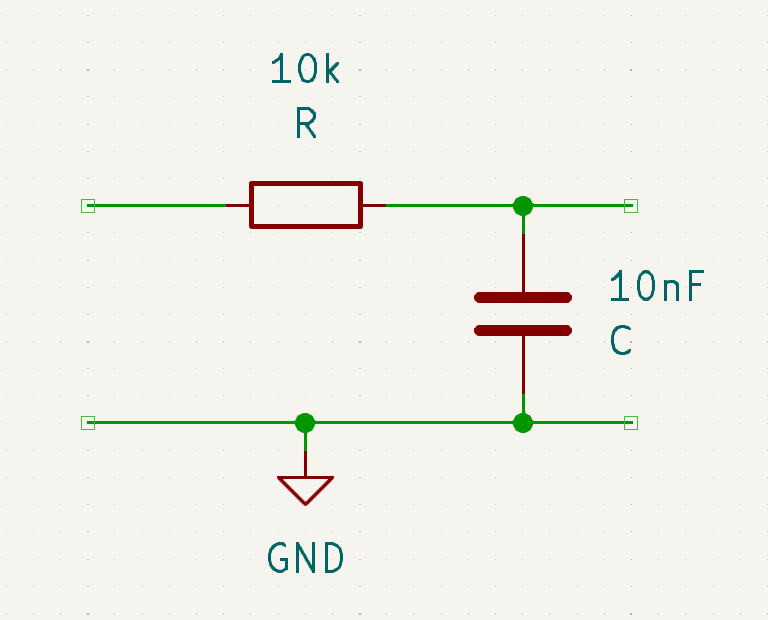
\includegraphics[height=.8\linewidth]{Images/RC-Tiefpass.png}
        \captionof{figure}{RC-Tiefpass}
        \label{RC_TP}
    \end{minipage}%
    \begin{minipage}{.5\textwidth}
        \centering
        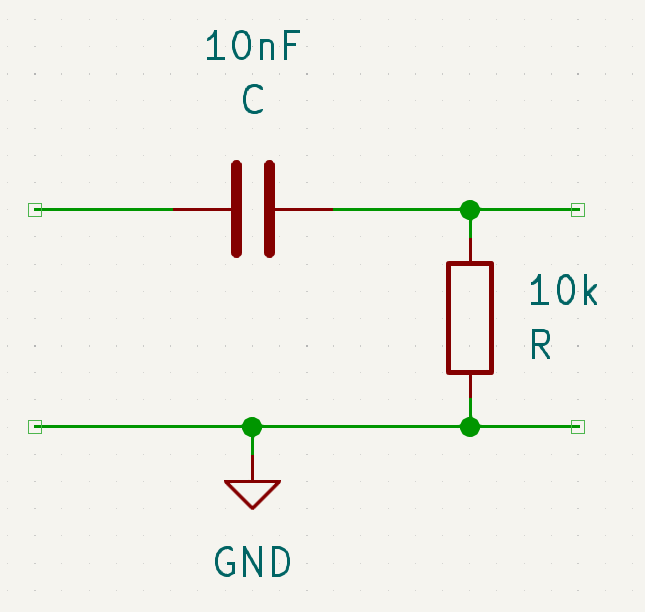
\includegraphics[height=.8\linewidth]{Images/RC-Hochpass.png}
        \captionof{figure}{RC-Hochpass}
        \label{RC_HP}
    \end{minipage}
\end{figure}
\noindent
Das Übertragungsverhältnis ist folgendermaßen definiert:
\begin{equation}
    \left\lvert G \right\rvert = \frac{\hat{U}_{\mathrm{out}}}{\hat{U}_{\mathrm{in}}}
\end{equation}
Die zugehörige Unsicherheit berechnet sich aus:
\begin{equation}
    \begin{split}
        \Delta \left\lvert G \right\rvert   &= \sqrt{\left(\frac{\partial \left\lvert G \right\rvert}{\partial \hat{U}_{\mathrm{out}}} \cdot \Delta \hat{U}_{\mathrm{out}}\right)^2 + \left(\frac{\partial \left\lvert G \right\rvert}{\partial \hat{U}_{\mathrm{in}}} \cdot \Delta \hat{U}_{\mathrm{in}}\right)^2} \\
                                            &= \sqrt{\left(\frac{\Delta \hat{U}_{\mathrm{out}}}{\hat{U}_{\mathrm{in}}}\right)^2 + \left(\frac{\hat{U}_{\mathrm{out}} \cdot \Delta \hat{U}_{\mathrm{in}}}{\hat{U}_{\mathrm{in}}^2}\right)^2} \\
                                            &= \left\lvert G \right\rvert \sqrt{\left(\frac{\Delta \hat{U}_{\mathrm{out}}}{\hat{U}_{\mathrm{out}}}\right)^2 + \left(\frac{\Delta \hat{U}_{\mathrm{in}}}{\hat{U}_{\mathrm{in}}}\right)^2}
    \end{split}
\end{equation}
\newpage \noindent
Für einen Tiefpass errechnet sich das Übertragungsverhältnis mithilfe der Maschenregel und Abb. \ref{RC_TP} folgendermaßen:
\begin{equation}
    \begin{split}
        \left\lvert G \right\rvert  &= \left\lvert \frac{Z_{out} \cdot I}{Z_{ges} \cdot I} \right\rvert \\
                                    &= \left\lvert \frac{\frac{1}{i\omega C}}{R + \frac{1}{i \omega C}} \right\rvert \\
                                    &= \left\lvert \frac{1}{i\omega RC + 1} \right\rvert \\
                                    &= \frac{1}{\sqrt{(\omega RC)^2 + 1}}
    \end{split}
    \label{eq:G_TP}
\end{equation}
Für einen Hochpass ergibt sich nach Abb. \ref{RC_HP}:
\begin{equation}
    \begin{split}
        \left\lvert G \right\rvert  &= \left\lvert \frac{Z_{out} \cdot I}{Z_{ges} \cdot I} \right\rvert \\
                                    &= \left\lvert \frac{R}{R + \frac{1}{i \omega C}} \right\rvert \\
                                    &= \left\lvert \frac{i \omega RC}{i \omega RC + 1} \right\rvert \\
                                    &= \frac{\omega RC}{\sqrt{(\omega RC)^2 + 1}}
    \end{split}
    \label{eq:G_HP}
\end{equation}
Eine charakteristische Größe des $\left\lvert B \right\rvert (\omega)$-Verlaufs ist die Grenzfrequenz ($\omega_g$). Bei dieser
Frequenz ist Übertragungsverhältnis auf $1/\sqrt{2}$ abgefallen. Da $P \propto U^2$ entspricht das einer Halbierung 
des Leistungsübertragungsverhältnis. Nach den Gleichungen \ref{eq:G_TP} und \ref{eq:G_HP} liegt die theoretische Grenzfrequenz
sowohl beim Tief- als auch beim Hochpass bei:
\begin{equation}
    \omega_g = \frac{1}{RC}
    \label{eq:omegaGrenz}
\end{equation}
\newpage
\subsection{Auswertung der experimentellen Daten}
Dies wollen wir nun mit den experimentell bestimmten werten vergleichen. 
\subsubsection{Tiefpass}
Wir behandeln hier zunächst den Tiefpass.
Die hier eingegebene Amplitude lag bei $U_1 = (1.090 \pm 0.013)\si{V}$.
Aus den frequenzabhängigen Amplituden konnten dann mithilfe eines Python Scripts (Siehe \ref{scr:UebertragungsverhaeltnisBerechnung}) folgende Übertragungs\-verhältnisse und Unsicherheiten 
errechnet werden:
\begin{table}[H]
    \centering
    \label{tab:TPAmps}
    \begin{tabular}{| c | c | c |}
        \hline
        Frequenz $f$ (in $\si{Hz}$) &  Amplitude am Ausgang $\hat{U}_{\mathrm{out}}$(in $V$) & Übertragungsverhältnis $\left\lvert G \right\rvert$\\
        \hline
        $100.00 \pm 0.10$ & $1.075 \pm 0.025$ & $0.986 \pm 0.026$ \\
        $500 \pm 10$ & $1.002 \pm 0.025$ & $0.919 \pm 0.025$ \\
        $1000.0 \pm 2.0$ & $0.890 \pm 0.025$ & $0.817 \pm 0.025$ \\
        $1200.0 \pm 2.0$ & $0.845 \pm 0.025$ & $0.775 \pm 0.025$ \\
        $1400.0 \pm 2.0$ & $0.770 \pm 0.025$ & $0.706 \pm 0.024$ \\
        $1600.0 \pm 2.0$ & $0.725 \pm 0.025$ & $0.665 \pm 0.024$ \\
        $1800.0 \pm 2.0$ & $0.680 \pm 0.005$ & $0.624 \pm 0.009$ \\
        $2000.0 \pm 2.0$ & $0.635 \pm 0.005$ & $0.583 \pm 0.008$ \\
        $2500.0 \pm 2.0$ & $0.545 \pm 0.005$ & $0.500 \pm 0.008$ \\
        $3000.0 \pm 2.0$ & $0.476 \pm 0.005$ & $0.437 \pm 0.007$ \\
        $4000.0 \pm 2.0$ & $0.379 \pm 0.005$ & $0.348 \pm 0.006$ \\
        $5000 \pm 10$ & $0.305 \pm 0.025$ & $0.280 \pm 0.023$ \\
        \hline
    \end{tabular}
    \caption{Ausgangsamplituden und Übertragungsverhältnisse eines Tiefpasses in Abhängigkeit von der Frequenz}
\end{table}
\noindent
Plottet man diese Werte und legt eine Kurve mit dem Ansatz $\left\lvert G \right\rvert(x) = b/\sqrt{a\omega^2 + 1}$ durch die Mittelwerte und jeweils durch die maximalen
positiven und negativen Abweichungen $\left\lvert G \right\rvert \pm \Delta \left\lvert G \right\rvert$ erhält man den Graphen \ref{fig:G_TP}. \\
Für $\omega \to 0$
verläuft der Graph ungefähr gegen einen Wert von $1$, für $\omega \to \infty$ strebt der Graph gegen einen kleinen Wert. Es ist allerdings nicht direkt ablesbar,
ob dieser Wert ein Übertragungsverhältnis von $0$ ist. \\
Sollte der Verlauf tatsächlich für $\omega \to \infty$ gegen $0$ streben, würde das experimentelle Ergebnis mit der theoretischen Vorhersage über 
einen Tiefpass übereinstimmen, denn aus der Theorie folgt (nach \ref{eq:G_TP}):
\begin{equation}
    \begin{split}
        \lim_{\omega \to 0} \left\lvert G_{\mathrm{TP}} \right\rvert &= \lim_{\omega \to 0} \frac{1}{\sqrt{\left(\omega RC\right)^2 + 1}} = 1 \\
        \lim_{\omega \to \infty} \left\lvert G_{\mathrm{TP}} \right\rvert &= \lim_{\omega \to \infty} \frac{1}{\sqrt{\left(\omega RC\right)^2 + 1}} = 0 \\
    \end{split}
\end{equation}
Aus dem Schnittpunkt der drei
Kurven mit der Geraden bei $\left\lvert G \right\rvert = 1/\sqrt{2}$ erhält man $\bar{f}_g$ sowie die Abweichung $\Delta f_g$.
Der bestimmte Wert für die Grenzfrequenz liegt damit bei:
\begin{equation}
    \begin{split}
        &\boxed{f_g = (1430 \pm 80) \si{Hz}} \\
        &\boxed{\omega_g = (9.0 \pm 0.5) \cdot 10^3 \cdot \si{\per \second}}
    \end{split}
    \label{eq:grfreqTP}
\end{equation}
\begin{figure}[H]
    \centering
    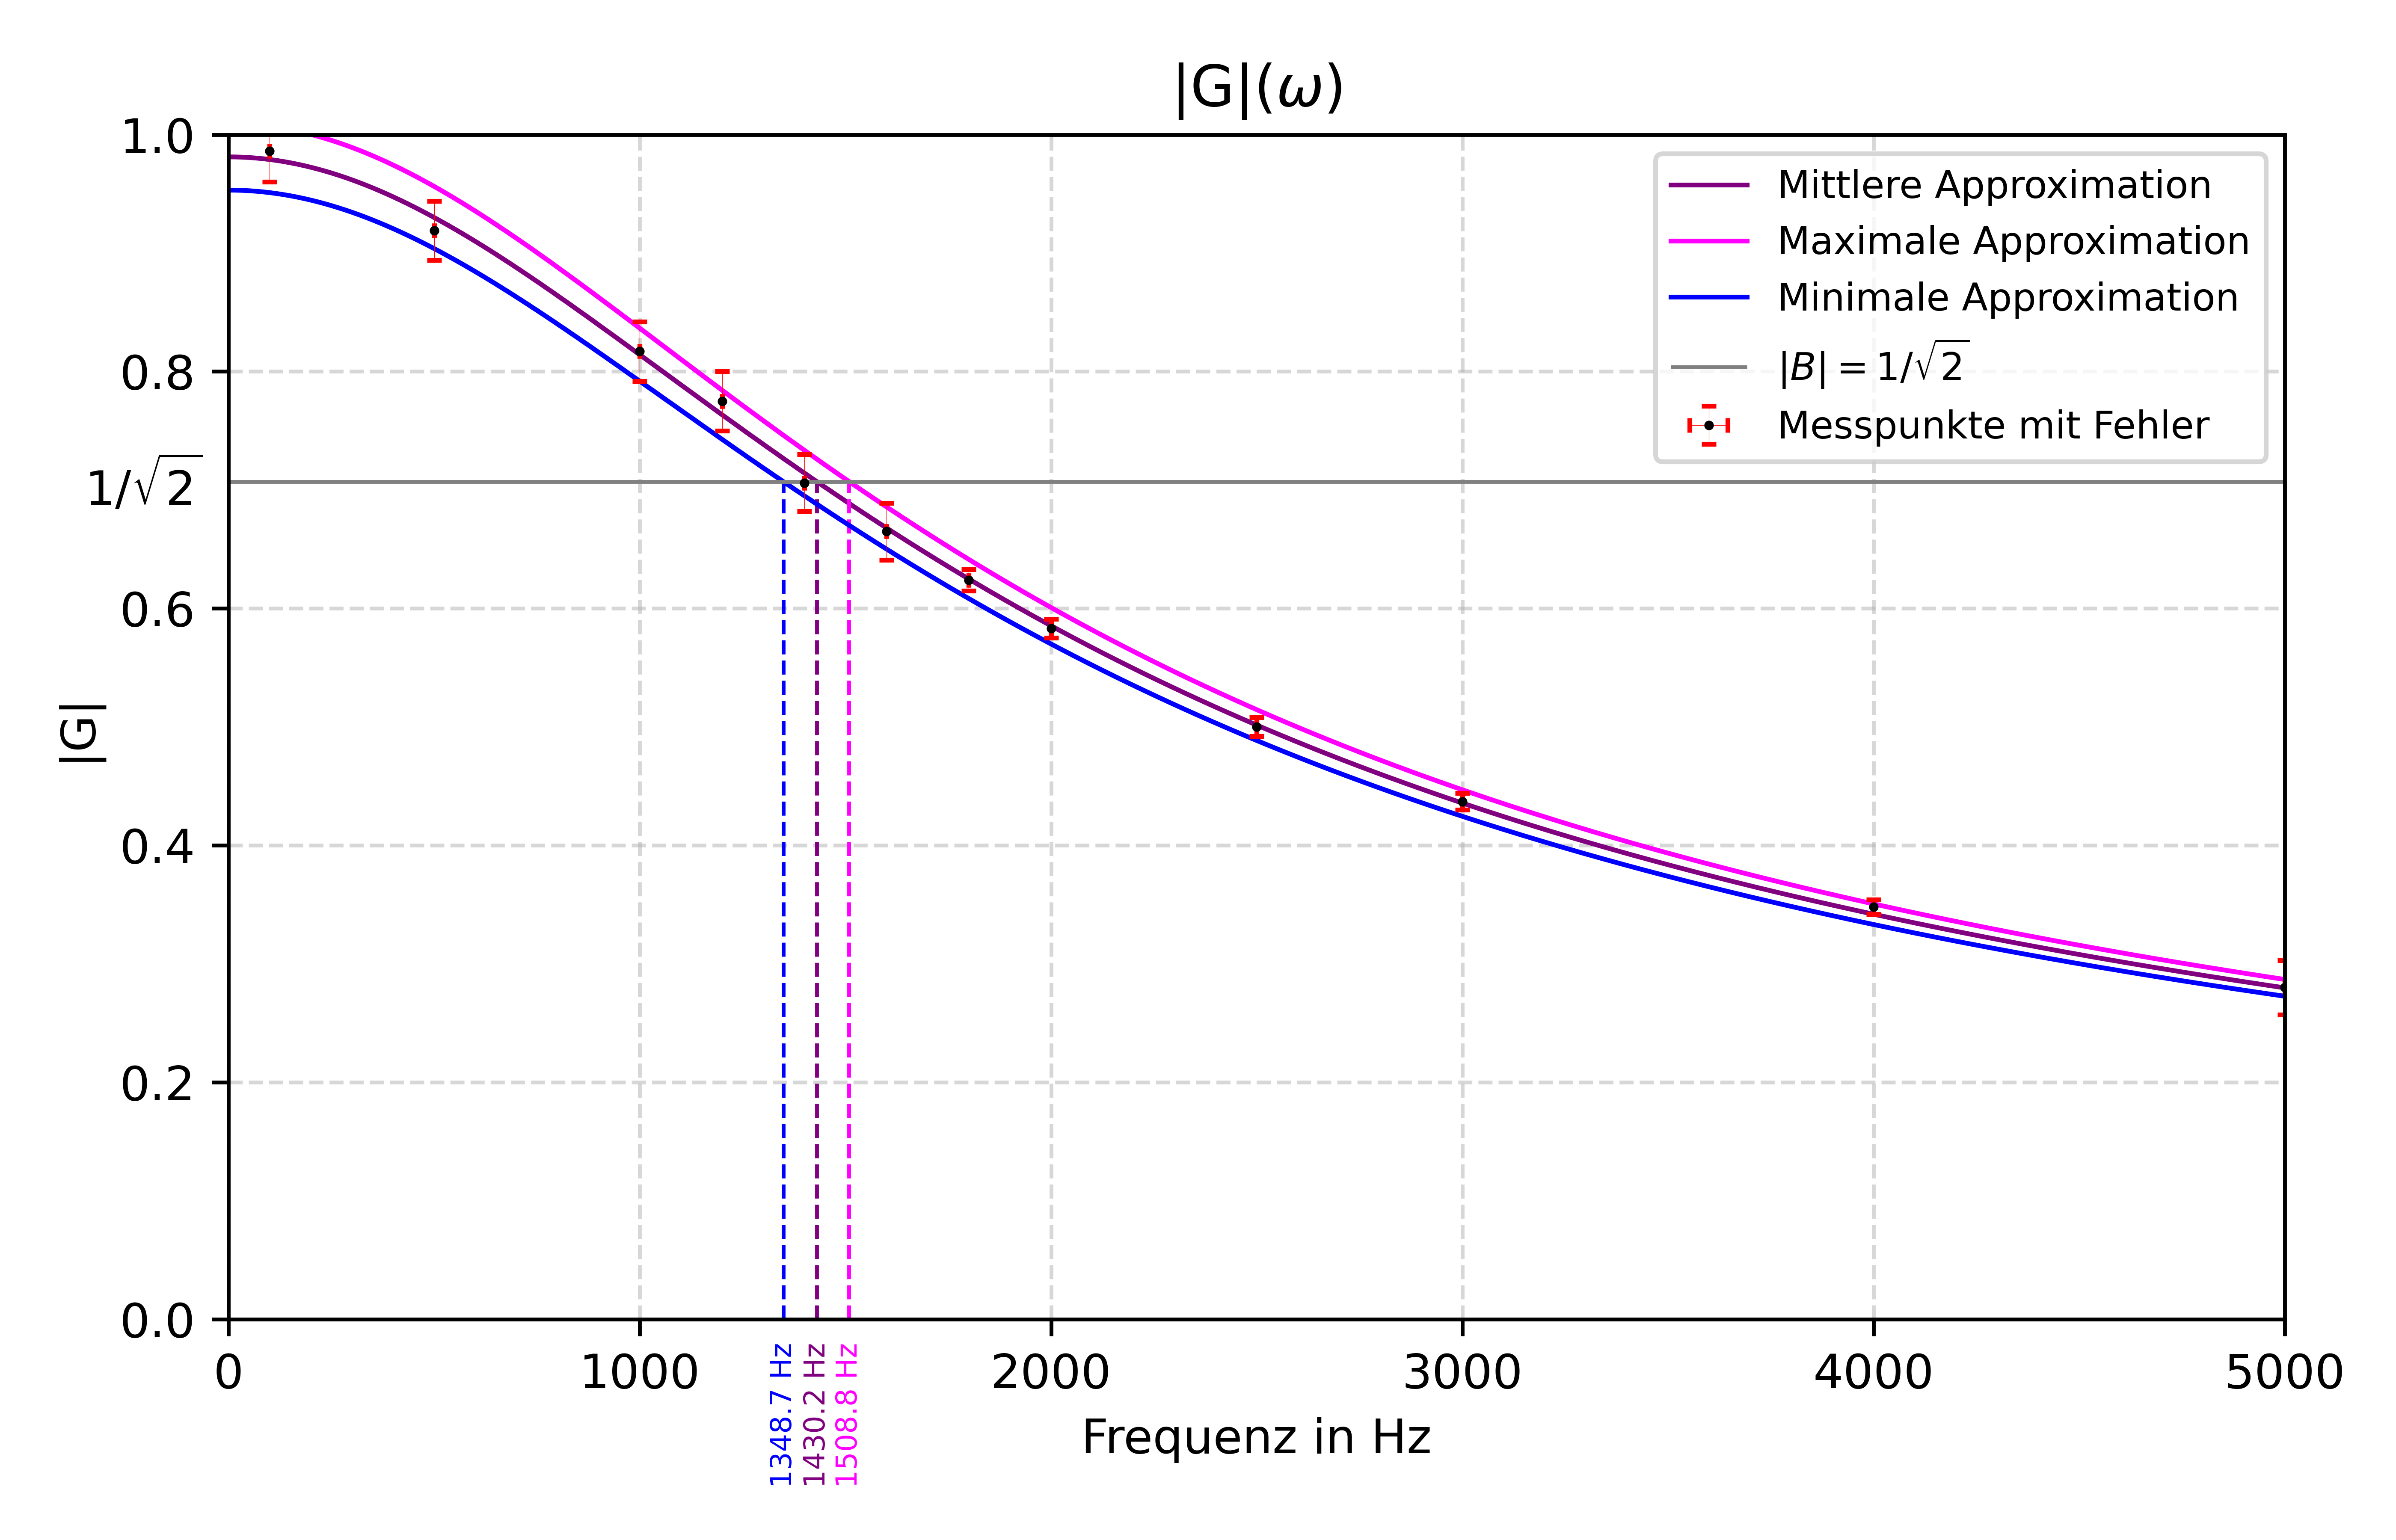
\includegraphics[width=1\textwidth]{./Images/UebertragungsverhaeltnisTP.png}
    \caption{Übertragungsverhältnisse eines Tiefpasses}
    \label{fig:G_TP}
\end{figure}
\subsubsection{Hochpass}
Nun betrachten wir den Hochpass. Hier wurde eine Amplitude von $U_{in} = (0.690 \pm 0.013) \si{V}$ angelegt. Äquivalent zum Tiefpass erhält man wieder mithilfe des Python Scripts folgende Werte:
\begin{table}[H]
    \centering
    \label{tab:HPAmps}
    \begin{tabular}{| c | c | c |}
        \hline
        Frequenz $f$ (in $\si{Hz}$) &  Amplitude am Ausgang $\hat{U}_{\mathrm{out}}$(in $V$) & Übertragungsverhältnis $\left\lvert G \right\rvert$\\
        \hline
        $100.00 \pm 0.10$ & $0.070 \pm 0.005$ & $0.101 \pm 0.007$ \\
        $500 \pm 10$ & $0.318 \pm 0.005$ & $0.461 \pm 0.011$ \\
        $1000.0 \pm 2.0$ & $0.378 \pm 0.005$ & $0.548 \pm 0.013$ \\
        $1200.0 \pm 2.0$ & $0.420 \pm 0.005$ & $0.609 \pm 0.014$ \\
        $1400.0 \pm 2.0$ & $0.462 \pm 0.005$ & $0.670 \pm 0.015$ \\
        $1640.0 \pm 2.0$ & $0.495 \pm 0.005$ & $0.717 \pm 0.015$ \\
        $1840.0 \pm 2.0$ & $0.525 \pm 0.005$ & $0.761 \pm 0.016$ \\
        $2000.0 \pm 2.0$ & $0.550 \pm 0.013$ & $0.797 \pm 0.024$ \\
        $2570.0 \pm 2.0$ & $0.590 \pm 0.013$ & $0.855 \pm 0.025$ \\
        $3000.0 \pm 2.0$ & $0.610 \pm 0.013$ & $0.884 \pm 0.025$ \\
        $4000.0 \pm 2.0$ & $0.640 \pm 0.013$ & $0.928 \pm 0.026$ \\
        $5000 \pm 2.0$ & $0.655 \pm 0.013$ & $0.949 \pm 0.026$ \\
        \hline
    \end{tabular}
    \caption{Ausgangsamplituden und Übertragungsverhältnisse eines Hochpasses in Abhängigkeit von der Frequenz}
\end{table}
\noindent
Für den Hochpass wurde der Plot (Abb. \ref{fig:G_HP}) mit dem Näherungsansatz $\left\lvert G \right\rvert(x) = b\omega/\sqrt{a\omega^2 + 1}$ erstellt.
Der Graph verläuft für $\omega \to 0$ gegen einen Wert von $0$, für $\omega \to \infty$ strebt der Graph ungefähr gegen $1$. \\
Dieses Verhalten stimmt mit der Theorie über einen Hochpass überein, denn nach dieser folgt ebenfalls (nach \ref{eq:G_HP}):
\begin{equation}
    \begin{split}
        \lim_{\omega \to 0} \left\lvert G_{\mathrm{HP}} \right\rvert &= \lim_{\omega \to 0} \frac{\omega RC}{\sqrt{\left(\omega RC\right)^2 + 1}} = 1 \\
        \lim_{\omega \to \infty} \left\lvert G_{\mathrm{HP}} \right\rvert &= \lim_{\omega \to \infty} \frac{\omega RC}{\sqrt{\left(\omega RC\right)^2 + 1}} = 0 \\
    \end{split}
\end{equation}
\begin{figure}[H]
    \centering
    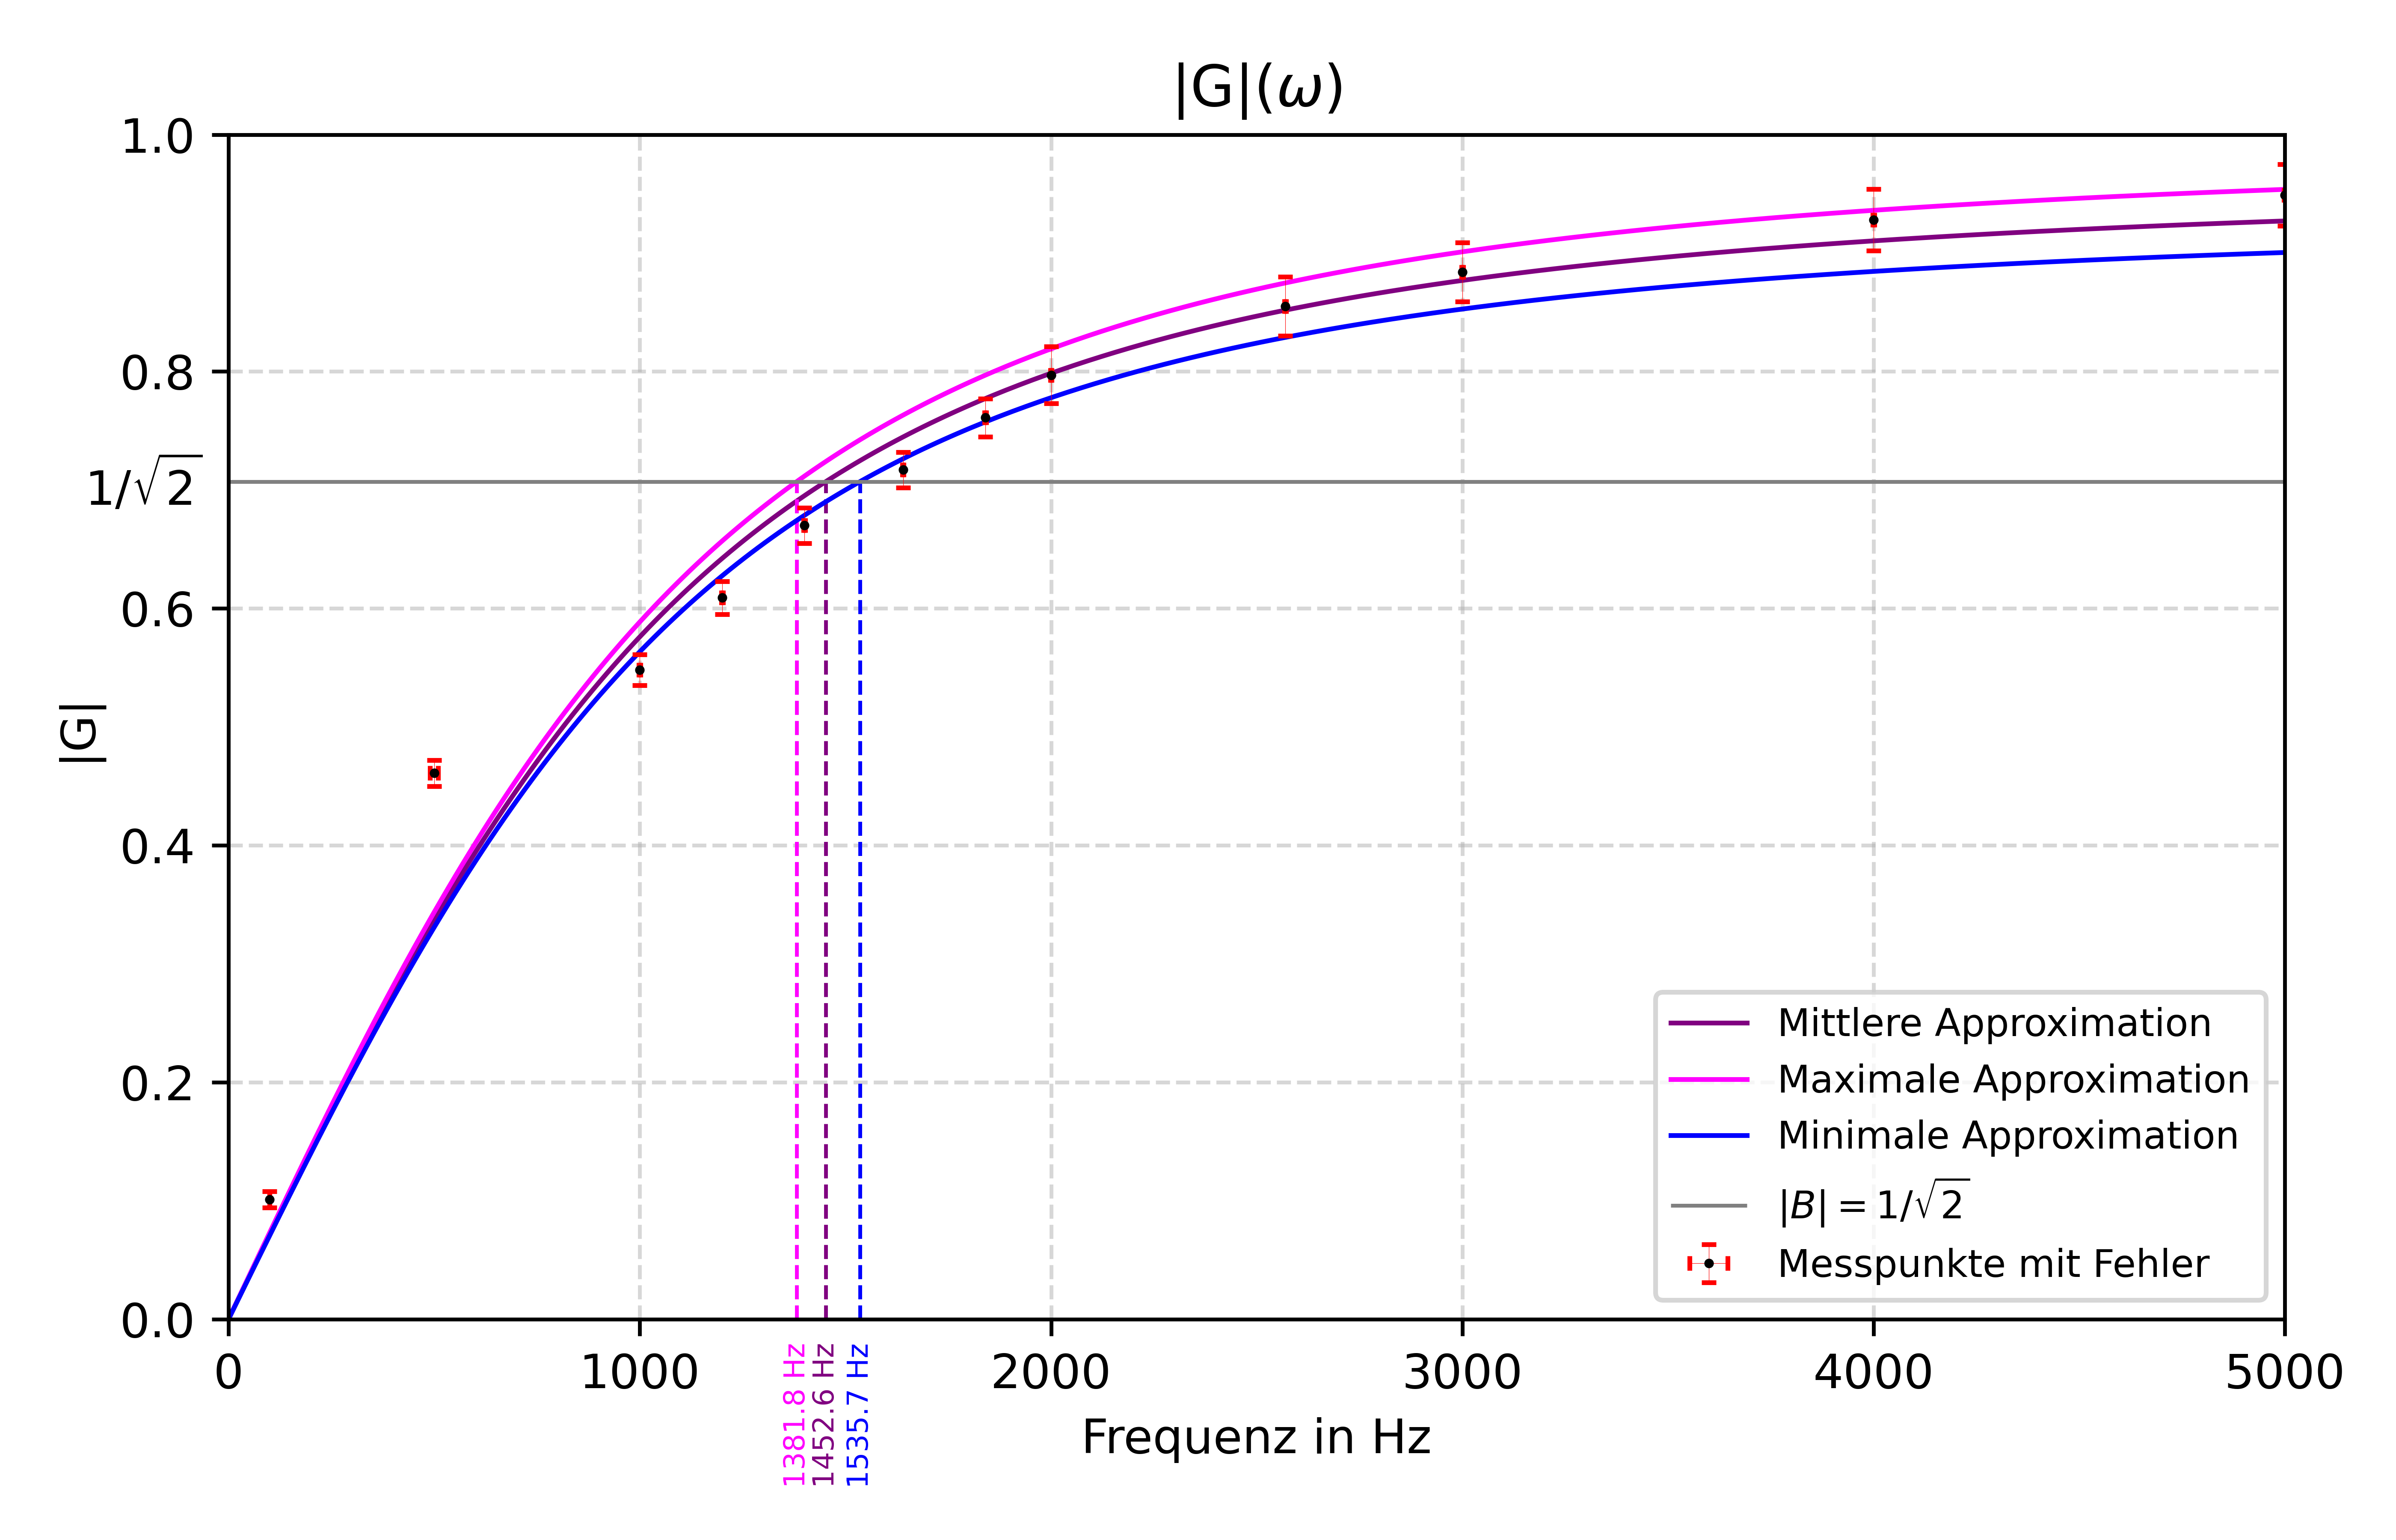
\includegraphics[width=1\textwidth]{./Images/UebertragungsverhaeltnisHP.png}
    \caption{Übertragungsverhältnisse eines Hochpasses}
    \label{fig:G_HP}
\end{figure}
Aus dem Graphen kann folgende Grenzfrequenz abgelesen werden:
\begin{equation}
    \begin{split}
        &\boxed{f_g = \qty{1450(90:70)}{Hz}} \\
        &\boxed{\omega_g = \qty{9.1(0.6:0.5)e3}{\per \second}}
    \end{split}
\end{equation}
Diese Werte stimmen im Rahmen der Messunsicherheit eindeutig mit den Werten des Hochpasses (\ref{eq:grfreqTP}) überein.
\subsubsection{Vergleich von Theorie und Experiment}
Zuletzt wollen wir noch die experimentell bestimmten Werte mit denjenigen vergleichen, die aus der Theorie folgen.
Nach Gleichung \ref{eq:omegaGrenz} gilt:
\begin{equation}
    \begin{split}
        \bar{\omega}_{\mathrm{g, theo}}     &= \frac{1}{\bar{R}\bar{C}} \\
                                            &= \qty{10e3}{1/s}
    \end{split}
\end{equation}
Wir nehmen die Unsicherheiten $\Delta R = 1\% R$ und $\Delta C = 1\% C$ an. Daraus ergibt sich die Unsicherheit der Grenzfrequenz aus der Gauß'schen Fehlerfortpflanzung.
\begin{equation}
    \begin{split}
        \Delta \omega_{\mathrm{g, theo}}    &= \sqrt{\left(\frac{\partial \omega_g}{\partial R}\Delta R\right)^2 + \left(\frac{\partial \omega_G}{\partial C}\Delta C\right)^2}\\
                                            &= \frac{1}{RC} \sqrt{\left(\frac{\Delta R}{R}\right)^2 + \left(\frac{\Delta C}{C}\right)^2} \\
                                            &= \qty{0.15e3}{1/s}
    \end{split}
\end{equation}
Damit ergäbe sich eine theoretische Grenzfrequenz von:
\begin{equation}
    \omega_{\mathrm{g, theo}} = (10.00 \pm 0.15) \times 10^3 \si{\per \second}
\end{equation}
Diese stimmt nicht mit der experimentell gemessenen Grenzfrequenz überein. Allerdings beruht sie auch auf einer sehr optimistischen Schätzung der Unsicherheit des 
Kondensators. Typische Folienkondensatoren, wie der im Versuch verwendete, weisen meist eher eine Unsicherheit im Bereich zwischen $5\%$ und $10\%$ auf. Nutzt man eine Abschätzung 
von $\Delta C = 5\%C$ erhält man: 
\begin{equation}
    \Delta \omega_{\mathrm{g, theo}} = \qty{0.6e3}{\per \second}
\end{equation}
Damit verändert sich die theoretische Grenzfrequenz auf:
\begin{equation}
    \boxed{\omega_{\mathrm{g, theo}} = (10.0 \pm 0.6) \times 10^3 \si{\per\second}}
\end{equation}
Diese realistischere Abschätzung der Unsicherheit der Kapazität führt dazu, dass die theoretische Grenzfrequenz im Rahmen der Unsicherheiten mit beiden experimentell bestimmten 
Grenzfrequenzen übereinstimmt.

\newpage
\section{Teilversuch III: Resonanzkurve eines Schwingkreises}
In Teilversuch III wurde die Resonanzkurve eines LC-Serienschwingkreises aufgezeichnet, um daraus die Resonanzfrequenz des Oszillators bestimmen zu können.
Folgender Schaltkreis wurde zur Messung genutzt:
\begin{figure}[H]
    \centering
    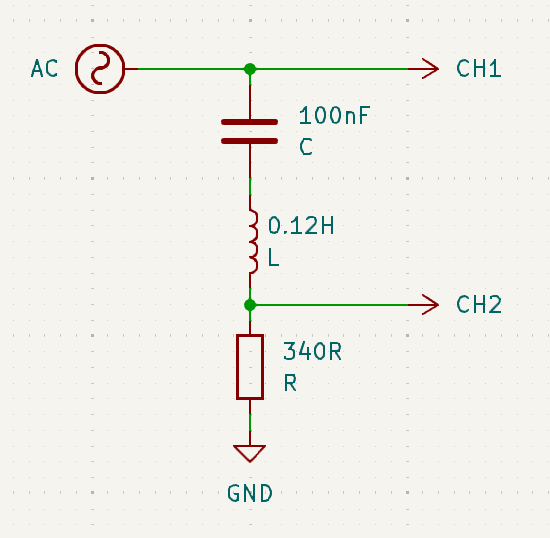
\includegraphics[width=0.5\textwidth]{./Images/LC-Schwingkreis.png}
    \caption{Gedämpfter LC-Schwingkreis}
    \label{fig:LCOsz}
\end{figure}
\subsection{Theoretischer Hintergrund}
Das Verhältnis zwischen Strom und Spannung in einem LC-Schwingkreis kann mithilfe eines komplexen Widerstands ($Z_\Sigma$) beschrieben werden. Mit diesem gilt:
\begin{equation}
    U(t) = Z_\Sigma I(t)
\end{equation}
Aus der Maschenregel folgt für $Z_\Sigma$:
\begin{equation}
    \begin{split}
        Z_\Sigma    &= Z_R + Z_C + Z_L \\
                    &= R - \frac{i}{\omega C} + i \omega L \\
                    &= R + i \frac{\omega^2 LC - 1}{\omega C}
    \end{split}
\end{equation}
Der Betrag des komplexen Widerstands ist damit gegeben durch:
\begin{equation}
    \left\lvert Z_{\Sigma} \right\rvert = \sqrt{R^2 + \left(\frac{\omega^2 LC - 1}{\omega C}\right)^2} = \frac{\hat{U}}{\hat{I}}
\end{equation}
Der komplexe Widerstand wird für eine bestimmte Frequenz minimal. Diese wird Resonanzfrequenz ($\omega_r$) genannt. Es gilt:
\begin{equation}
    \omega_r = \frac{1}{\sqrt{LC}}
    \label{eq:OmegarTheo}
\end{equation}
Bei dieser Frequenz wird der Imaginärteil des komplexen widerstands $0$ und somit der komplexe widerstand minimal, da der Realteil nicht von $\omega$ abhängt.
Bei $\omega_r$ ist also $\left\lvert Z_\Sigma \right\rvert = R$.
Bei gegebener Spannungsamplitude wird hier die Stromamplitude maximal.
Die Unsicherheit der so bestimmten Resonanzfrequenz berechnet sich folgendermaßen:
\begin{equation}
    \begin{split}
        \Delta \omega_r &= \sqrt{\left(\frac{\partial \omega_r}{\partial L} \Delta L\right)^2 + \left(\frac{\partial \omega_r}{\partial C} \Delta C\right)^2} \\
                        &= \frac{1}{2} \omega_r \sqrt{\left(\frac{\Delta L}{L}\right)^2 + \left(\frac{\Delta C}{C}\right)^2}
    \end{split}
    \label{eq:unsOmegarTheo}
\end{equation}

\subsection{Auswertung der experimentellen Daten}
Im Versuch wurde bei verschiedenen Frequenzen die Amplitude der Spannung $\hat{U}_R$ gemessen, die über den Widerstand abfällt. Diese ist über $\hat{I} = \frac{\hat{U}_R}{R}$ direkt mit der
Amplitude der Stromstärke gekoppelt.
Der fehler der Stromamplitude ergibt sich aus:
\begin{equation}
    \begin{split}
        \Delta \hat{I}  &= \sqrt{\left(\frac{\partial \hat{I}}{\partial \hat{U}} \Delta \hat{U}\right)^2 + \left(\frac{\partial \hat{I}}{\partial R} \Delta R\right)^2} \\
                        &= \frac{\hat{U}}{R} \sqrt{\left(\frac{\Delta \hat{U}}{\hat{U}}\right)^2 + \left(\frac{\Delta R}{R}\right)^2}
    \end{split}
\end{equation}
Hierbei wurden folgende Messwerte bestimmt:
\begin{table}[H]
    \centering
    \caption{Amplitude des Stroms bei verschiedenen Eingangsfrequenzen}
    \label{tab:IAmpfWerte}
    \begin{tabular}{c c c}
        \hline
        Frequenz in $\si{\kilo \hertz}$ & $\hat{U}_R$ in $\si{V}$ & $\hat{I}$ in  \\
        \hline
        $3.000 \pm 0.020$ & $0.168 \pm 0.025$ & $0.494 \pm 0.076$ \\
        $4.000 \pm 0.020$ & $0.554 \pm 0.025$ & $1.629 \pm 0.082$ \\
        $4.420 \pm 0.020$ & $1.040 \pm 0.025$ & $3.059 \pm 0.072$ \\
        $4.450 \pm 0.020$ & $1.040 \pm 0.025$ & $3.059 \pm 0.072$ \\
        $4.520 \pm 0.020$ & $1.000 \pm 0.025$ & $2.941 \pm 0.071$ \\
        $5.000 \pm 0.020$ & $0.520 \pm 0.025$ & $1.529 \pm 0.079$ \\
        $6.000 \pm 0.020$ & $0.225 \pm 0.025$ & $0.662 \pm 0.117$ \\
        \hline
    \end{tabular}
\end{table}
Plottet man diese Messwerte und legt eine Kurve hindurch, erhält man folgendes:
\begin{figure}[H]
    \centering
    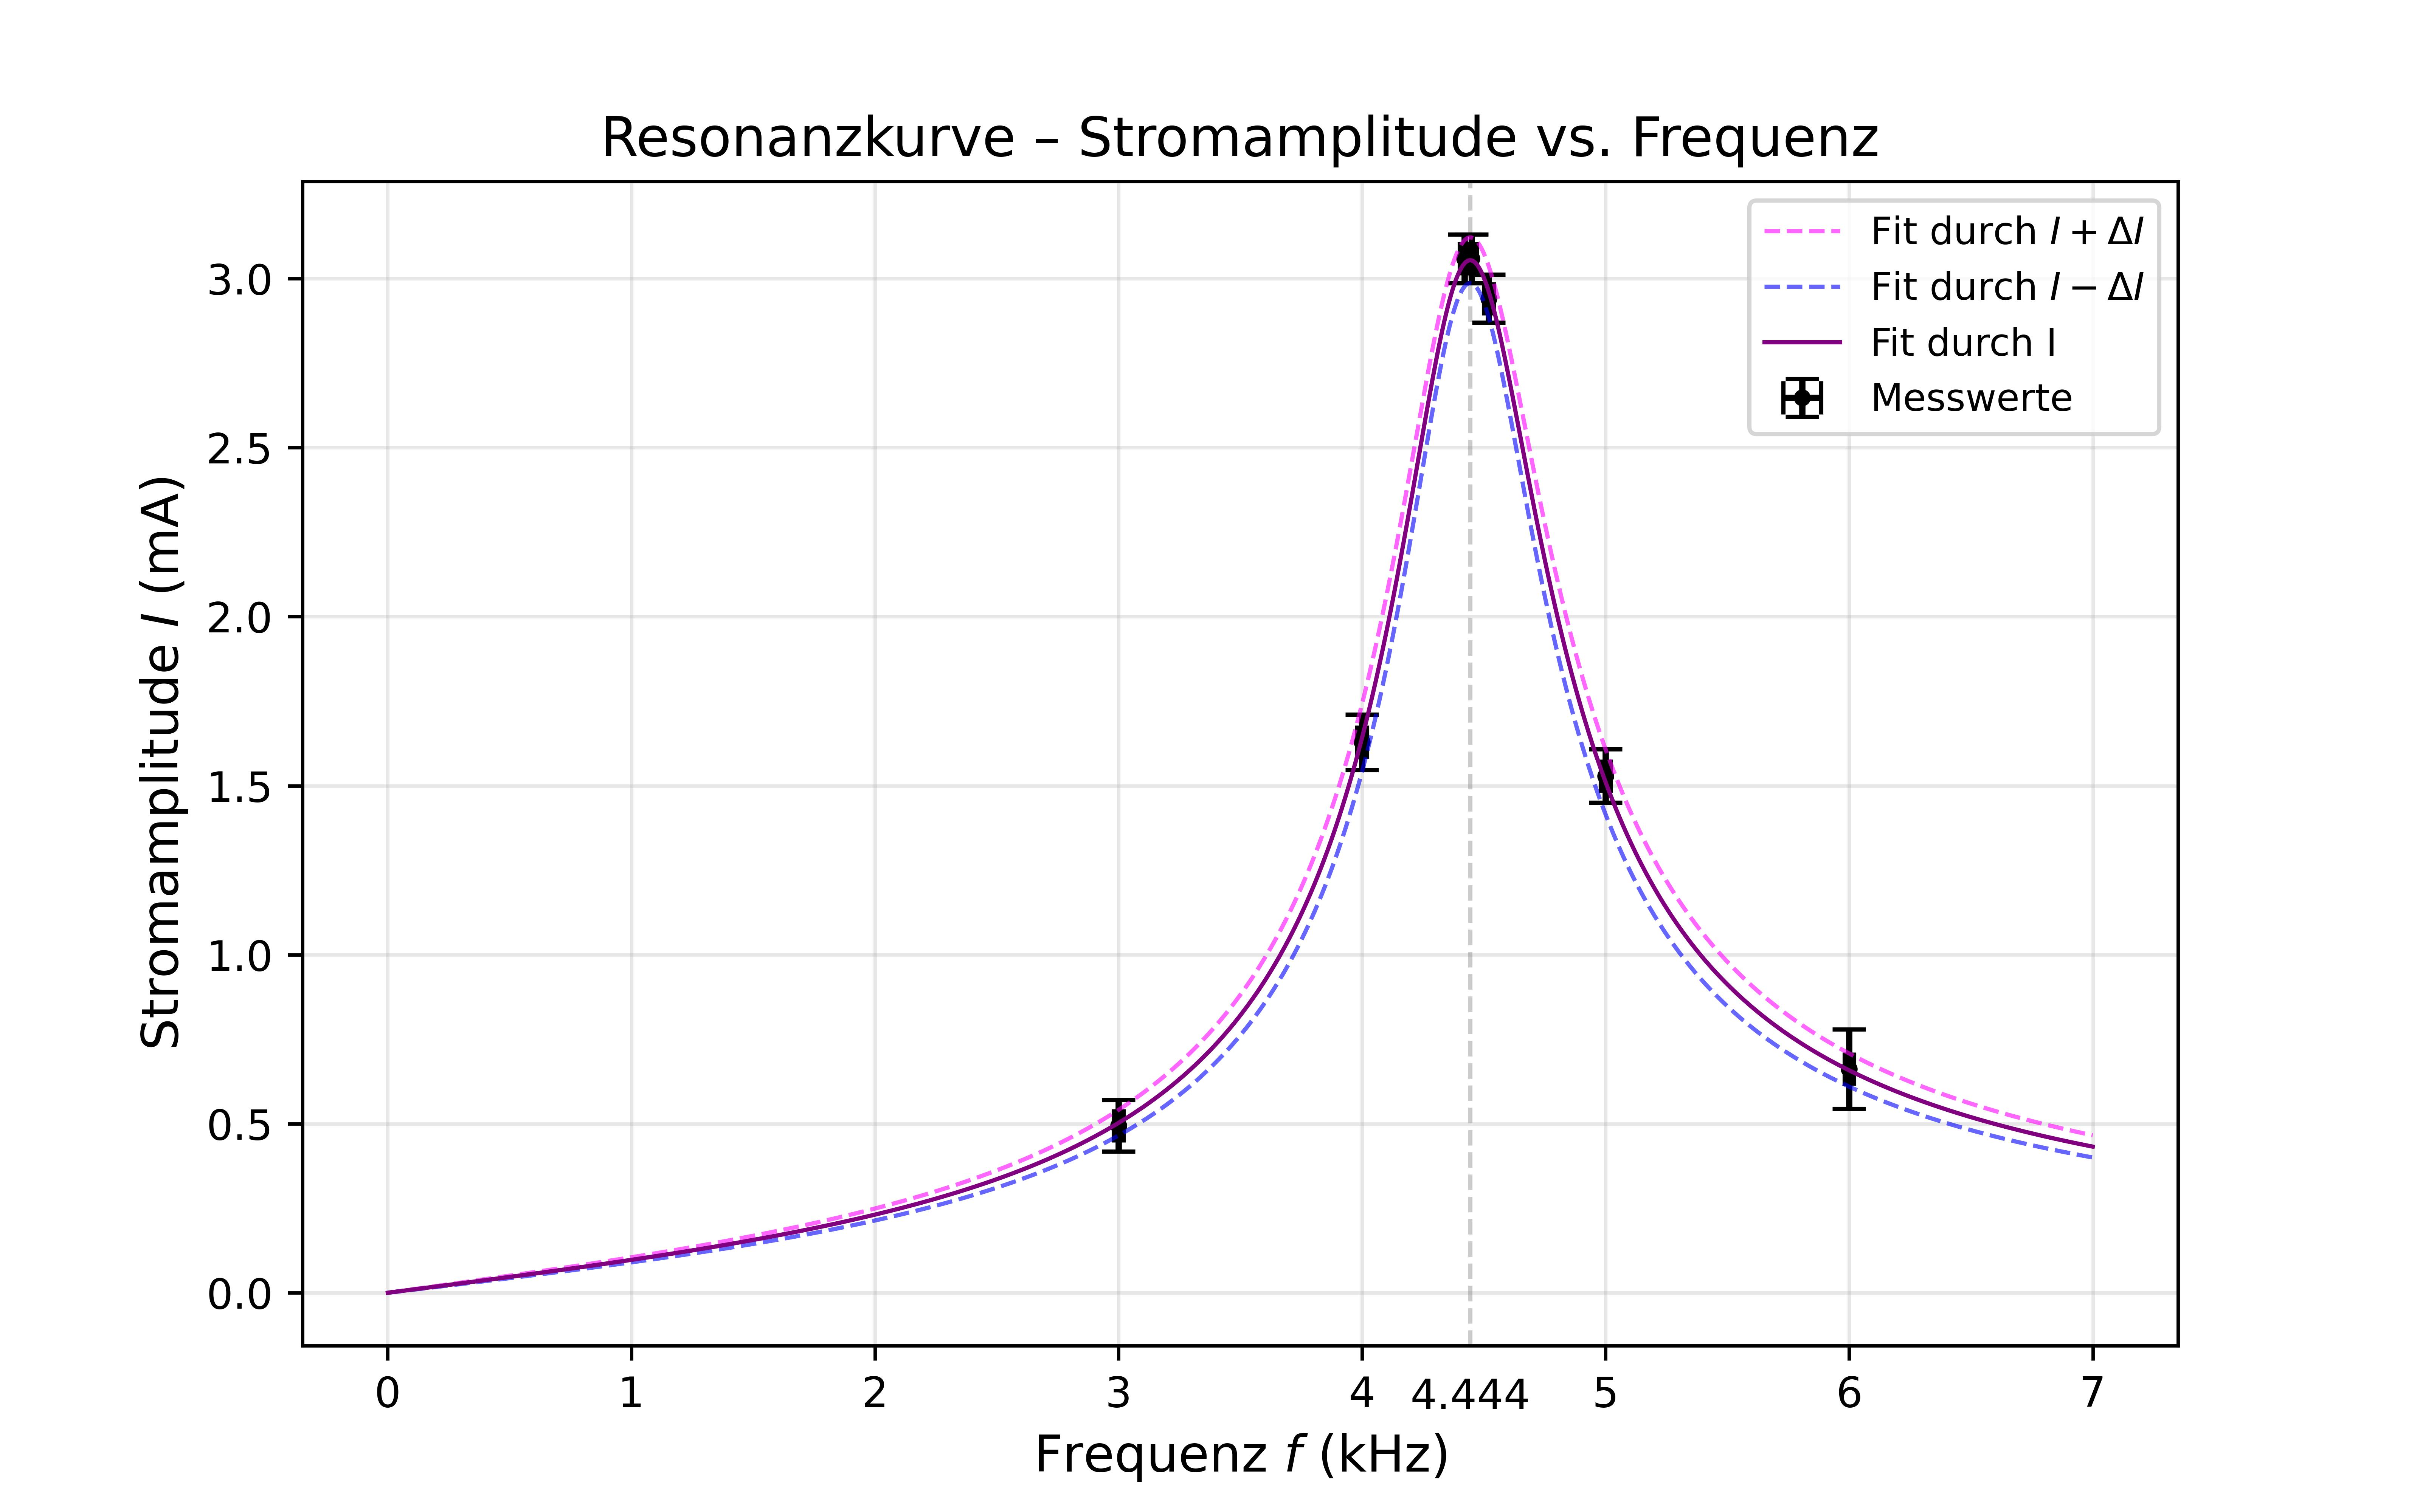
\includegraphics[width=1\textwidth]{./Images/Resonanzkurve.jpg}
    \caption{Resonanzkurve des Serienschwingkreises}
    \label{fig:ResSchwingkreis}
\end{figure}
\noindent
Die hiermit bestimmte Resonanzfrequenz liegt also bei:
\begin{equation}
    \begin{split}
        \boxed{f_r = (4.444 \pm 0.020) \si{\kilo\hertz}} \\
        \boxed{\omega_r = (27.92 \pm 0.13) \times 10^3 \si{\per\second}}
    \end{split}
\end{equation}
Berechnet man die Resonanzfrequenz aus der Theorie (Siehe \ref{eq:OmegarTheo} und \ref{eq:unsOmegarTheo}) mit $L = 0.120 \si{H} \pm 5\%L$ und $C = 10 \si{nF} \pm 5\%C$ erhält man:
\begin{equation}
    \boxed{\omega_{\mathrm{r, theo}} = (28,9 \pm 1.1) \times 10^3 \si{\per\second}}
\end{equation}
Somit stimmt der theoretisch berechnete Wert im Rahmen der Messungenauigkeit mit dem experimentell bestimmten Wert überein.
\subsection{Spannungseinbruch bei der Resonanzfrequenz}
Während des Versuchs wurde beobachtet, dass die Amplitude der Eingansspannung bei Frequenzen sehr nahe der Resonanzfrequenz geringfügig im vergleich zur ansonsten ziemlich konstanten Spannung 
einbrach. Dies lässt sich folgendermaßen erklären:
Beim Funktionsgenerator, der als Spannungsquelle dient, handelt es sich um eine reale Spannungsquelle. Diese hat einen Innenwiderstand $R_{\mathrm{innen}} > 0$.
Für Frequenzen nahe der Resonanzfrequenz lässt sich die Schaltung näherungsweise durch folgendes Ersatzschaltbild beschreiben, 
da der Imaginärteil des komplexen Widerstands aus Spule und Kondensator hier ungefähr bei $0$ liegt:
\begin{figure}[H]
    \centering
    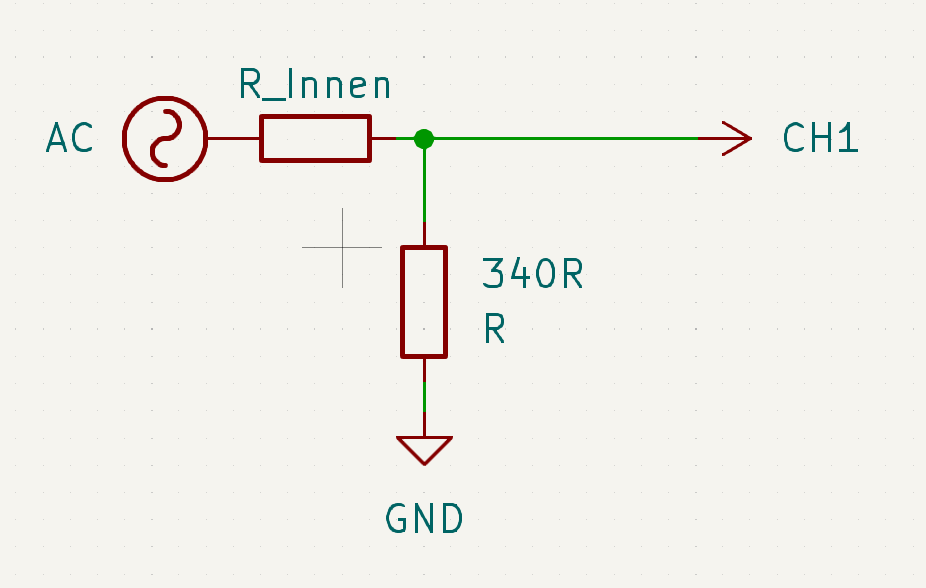
\includegraphics[width=.6\textwidth]{./Images/ErsatzschaltbildSpannungsteiler.png}
    \caption{Ersatzschaltbild mit Innenwiderstand des Funktionsgenerators}
    \label{fig:ErsSchaltbildFktGenerator}
\end{figure}
\noindent
Damit bilden der Innenwiderstand des Funktionsgenerators und der Widerstand $R$ einen Spannungsteiler, wodurch die gemessene Spannungsamplitude geringer ist. Für Frequenzen, die nicht 
in der Nähe der Resonanzfrequenz verlaufen wird zwar auch ein (in diesem Fall komplexer) Spannungsteiler gebildet, allerdings ist der Scheinwiderstand der Spule bzw. des Kondensators in diesen Fällen
so groß, dass $R_{\mathrm{innen}}$ im Vergleich vernachlässigbar klein ist und somit näherungsweise die gesamte Spannung über $Z_\Sigma$ abfällt.
\newpage
\section{Teilversuch IV: }

\newpage
\chapter{Anhang}
\section{Python Scripts}
Die Python Scripts, die zum Plotten der Grafiken verwendet wurden, wurden mit Unterstützung von KI erstellt und dann nach den eigenen Bedürfnissen weiter
bearbeitet.
\definecolor{codegreen}{rgb}{0,0.6,0}
\definecolor{codegray}{rgb}{0.5,0.5,0.5}
\definecolor{codepurple}{rgb}{0.58,0,0.82}
\definecolor{backcolour}{rgb}{0.95,0.95,0.92}
\lstdefinestyle{python}{
    backgroundcolor=\color{backcolour},   
    commentstyle=\color{codegreen},
    keywordstyle=\color{magenta},
    numberstyle=\tiny\color{codegray},
    stringstyle=\color{codepurple},
    basicstyle=\ttfamily\footnotesize,
    breakatwhitespace=false,         
    breaklines=true,                 
    captionpos=b,                    
    keepspaces=true,                 
    numbers=left,                    
    numbersep=5pt,                  
    showspaces=false,                
    showstringspaces=false,
    showtabs=false,                  
    tabsize=2
}
\subsection{TV II:}
\subsubsection{Berechnung der Übertragungsverhältnisse}
\label{scr:UebertragungsverhaeltnisBerechnung}
\begin{scriptsize}
\lstset{style=python}
\begin{lstlisting}[language=python]
import numpy as np
U_in  = 1.090
dU_in = 0.013
data = [
    ("100.00",  "0.10",  1.075, 0.025),
    ("500",     "10",    1.002, 0.025),
    ("1000.0",  "2.0",   0.890, 0.025),
    ("1200.0",  "2.0",   0.845, 0.025),
    ("1400.0",  "2.0",   0.770, 0.025),
    ("1600.0",  "2.0",   0.725, 0.025),
    ("1800.0",  "2.0",   0.680, 0.005),
    ("2000.0",  "2.0",   0.635, 0.005),
    ("2500.0",  "2.0",   0.545, 0.005),
    ("3000.0",  "2.0",   0.476, 0.005),
    ("4000.0",  "2.0",   0.379, 0.005),
    ("5000",    "10",    0.305, 0.025),
]
for f_str, df_str, U_out, dU_out in data:
    G  = U_out / U_in
    dG = G * np.sqrt((dU_out / U_out)**2 + (dU_in / U_in)**2)
    G_r  = round(G,  3)
    dG_r = round(dG, 3)
    row = (
        f"        ${f_str} \\pm {df_str}$"
        f" & ${U_out:.3f} \\pm {dU_out:.3f}$"
        f" & ${G_r:.3f} \\pm {dG_r:.3f}$ \\\\"
    )

    print(row)

\end{lstlisting}
\end{scriptsize}

\subsubsection{Übertragungsverhältnis Plot}
\label{scr:UebertragungsverhaeltnisPlot}
\begin{scriptsize}
\lstset{style=python}
\begin{lstlisting}[language=python]
import matplotlib.pyplot as plt
import numpy as np
from scipy.optimize import curve_fit, root_scalar 

G_grenz = 1/np.sqrt(2)
frequenz     = [100, 500, 1000, 1200, 1400, 1600, 1800, 2000, 2500, 3000, 4000, 5000]
g_mid = [0.986, 0.919,  0.817,  0.775,  0.706,  0.665,  0.624,  0.583,  0.500, 0.437, 0.348, 0.280]
freq_err = [0.025, 0.025, 0.025, 0.025, 0.025, 0.025, 0.005, 0.005, 0.005, 0.005, 0.005, 0.025]
g_err = [0.026, 0.025, 0.025, 0.025, 0.024, 0.024, 0.009, 0.008, 0.008, 0.007, 0.006, 0.023]
g_max = np.array(g_mid) + np.array(g_err)
g_min = np.array(g_mid) - np.array(g_err)
g_values = [(g_mid, "Mittlere Approximation", "purple"), (g_max, "Maximale Approximation", "magenta"), (g_min, "Minimale Approximation", "blue")]
def f(x, a, b):
    return b/np.sqrt(a * x**2 + 1)

fig, ax = plt.subplots(figsize=(7, 4.5))
freq_fit = np.linspace(0, 5000, 300)

for g, label, color in g_values:
    popt, pcov = curve_fit(f, frequenz, g, p0=[1.0, 1.0])
    a, b = popt[0], popt[1]
    ax.plot(freq_fit, f(freq_fit, a, b), color = color, linewidth = 1, label = label)
    res = root_scalar(lambda x: f(x, a, b) - G_grenz, bracket=[0, 5000])
    plt.vlines(res.root, 0, G_grenz, linewidth = .8, linestyles="--", color = color)
    plt.text(res.root, -0.02, f'{res.root:.1f} Hz',
         ha='center', va='top', rotation=90, color = color, fontsize = 6)

plt.hlines(G_grenz, 0, 5000, color = "grey", linewidth = .8, label=r"$|B| = 1/\sqrt{2}$")

ax.errorbar(frequenz, g_mid, xerr=freq_err, yerr=g_err, fmt='o', ms = '1', mec = 'black',  
            ecolor='red', elinewidth=.1, capsize=1.5, label="Messpunkte mit Fehler")

ax.set_xlabel("Frequenz in Hz")
ax.set_ylabel("|G|")
ax.set_title(r"|G|($\omega$)")
ax.legend(fontsize = 8)
ax.grid(True, linestyle="--", alpha=0.5)
ax.set_xlim(0, 5000)
ax.set_ylim(0, 1)
# plt.show()

plt.tight_layout()
plt.savefig("./02_VPO/Images/UebertragungsverhaeltnisTP.png", dpi=800)
\end{lstlisting}
\end{scriptsize}

\subsection{TV III:}
\subsubsection{Resonanzkurve Plot}
\label{scr:ResonanzkurvePlot}
\begin{scriptsize}
\lstset{style=python}
\begin{lstlisting}[language=python]
import numpy as np
import matplotlib.pyplot as plt
from scipy.optimize import curve_fit

f     = np.array([3.000, 4.000, 4.420, 4.450, 4.520, 5.000, 6.000])  # kHz
df    = np.array([0.02,  0.02,  0.02,  0.02,  0.02,  0.02,  0.02 ])

I     = np.array([0.494, 1.629, 3.059, 3.059, 2.941, 1.529, 0.662])   # mA
dI    = np.array([0.076, 0.082, 0.072, 0.072, 0.071, 0.079, 0.117])

def resonance(f, I_max, f0, Q):
    return I_max / np.sqrt(1 + Q**2 * (f/f0 - f0/f)**2)

p0 = [3.0, 4.43, 5.0]

popt,  pcov  = curve_fit(resonance, f, I,      p0=p0, sigma=dI, absolute_sigma=True)
# Fit durch I + dI
popt_up, _   = curve_fit(resonance, f, I + dI, p0=p0, sigma=dI, absolute_sigma=True)
# Fit durch I - dI
popt_dn, _   = curve_fit(resonance, f, I - dI, p0=p0, sigma=dI, absolute_sigma=True)

perr = np.sqrt(np.diag(pcov))
I_max_fit, f0_fit, Q_fit = popt
dI_max, df0, dQ          = perr

f_fine = np.linspace(0, 7.0, 1000)

fig, ax = plt.subplots(figsize=(8, 5))
ax.errorbar(f, I, xerr=df, yerr=dI,
            fmt='.', color='black', capsize=4,
            label='Messwerte', zorder=3)

ax.plot(f_fine, resonance(f_fine, *popt_up), color='magenta', lw=1,
        ls='--', alpha=0.6, label='Fit durch $I + \\Delta I$', zorder = 5)
ax.plot(f_fine, resonance(f_fine, *popt_dn), color='blue', lw=1,
        ls='--',  alpha=0.6, label='Fit durch $I - \\Delta I$', zorder = 5)

ax.plot(f_fine, resonance(f_fine, *popt), color='purple', lw=1,
        label=(f'Fit durch I'), zorder = 5)

# Messwerte
ax.axvline(f0_fit, color='grey', lw=1, ls='--', alpha=0.4)
plt.text(f0_fit, -0.25, f"{f0_fit:.3f}", ha='center', va='top', color = "black", fontsize = 10)

ax.set_xlabel('Frequenz $f$ (kHz)', fontsize=12)
ax.set_ylabel('Stromamplitude $I$ (mA)', fontsize=12)
ax.set_title('Resonanzkurve – Stromamplitude vs. Frequenz', fontsize=13)
ax.legend(fontsize=9)
ax.grid(True, alpha=0.3)

# plt.tight_layout()
plt.savefig('./02_VPO/Images/Resonanzkurve.jpg', dpi=800)
\end{lstlisting}
\end{scriptsize}


\end{document}
